% !TEX root = ../main.tex
\documentclass[../main.tex]{subfiles}
\begin{document}


\subsection{Програмное обеспечение для микроконтроллера Arduino Due}

Микроконтроллер Arduino Due делает следующие операции:
\begin{itemize}
    \item собирает данные с микрофона
    \item издает звуковые импульсы через динамик
    \item собирает данные с двух датчиков давления bmp280
    \item передает эти данные через usb на компьютер
\end{itemize}


\subsubsection{Сбор данных с микрофона}
Микрофон подсоединяется к пину \texttt{A0} микроконтроллера. Напряжение с этого пина считывается и передается в АЦП/ADC преобразуясь в числа. Далее микроконтроллер считывает данные с АЦП и передает их через USB на компютер.

В начале программы инициализируется буффер в который будет производится запись полученных данных с АЦП:

\begin{lstlisting}
volatile int bufn, obufn;
uint16_t buf[4][256];   // 4 buffers of 256 readings
\end{lstlisting}

АЦП инициализируется следующим кодом:

\begin{lstlisting}
void init_adc() {
    pmc_enable_periph_clk(ID_ADC);
    adc_init(ADC, SystemCoreClock, ADC_FREQ_MAX, ADC_STARTUP_FAST);
    ADC -> ADC_MR |= 0x80; // free running

    ADC -> ADC_CHER = 0x80;

    NVIC_EnableIRQ(ADC_IRQn);
    ADC -> ADC_IDR = ~(1 << 27);
    ADC -> ADC_IER = 1 << 27;
    ADC -> ADC_RPR = (uint32_t)buf[0]; // DMA buffer
    ADC -> ADC_RCR = 256;
    ADC -> ADC_RNPR = (uint32_t)buf[1]; // next DMA buffer
    ADC -> ADC_RNCR = 256;
    bufn = obufn = 1;
    ADC -> ADC_PTCR = 1;
    ADC -> ADC_CR = 2;
}
\end{lstlisting}

Код выше переводит АЦП в режим Free Running Mode. Это самый быстрый режим работы данного АЦП. Его особенность заключается в том, что нет необходимости вручную собирать данные через определенное количество времени. Программа пользователя запускает только первый сбор данных, а дальше АЦП сам автоматически начинает преобразование сразу как только закончилось предыдущее. Таким образом не возникает простоев АЦП и не теряются данные.

Cтоит отметить включение режима прямого доступа к памяти микроконтроллера AT91S-AM3X8E (DMA: Direct Memory Access). Этот режим позволяет обращаться напрямую к памяти микроконтроллера, таким образом не отнимая процессорное время самого микроконтроллера. Процессор не прерывается на обработку запроса к памяти и постоянно занят сбором данных с АЦП. Это позволяет приблизится к максимальной частоте дискретизации.

АЦП записывает данные в буфферы DMA. Отуда они идут в переменную \texttt{buf}. Переменная \texttt{buf} это двухмерный массив размером (4, 256): запись производится циклически в эти 4 массива.
Функция которая периодически сдвигает буфферы выглядит так:

\begin{lstlisting}
void ADC_Handler() {    // move DMA pointers to next buffer
    int f = ADC -> ADC_ISR;
    if (f & (1 << 27)) {
        bufn = (bufn + 1) & 3;
        ADC -> ADC_RNPR = (uint32_t)buf[bufn];
        ADC -> ADC_RNCR = 256;
    }
}
\end{lstlisting}

Эта функция вызывается в стандартной для Arduino функции \texttt{setup()}:


\begin{lstlisting}
void setup() {
    
    // ...
    
    init_adc();
}
\end{lstlisting}



В стандартной для Arduino функции \texttt{loop()} происходит ожидание пока буфер заполнится. Буффер содержит значения типа данных \texttt{uint16\_t}. Чтобы передать данные через USB при помощи функции \texttt{SerialUSB.write} данные преобразуются в байты.
Также производится увеличение переменной \texttt{obufn}, означающее что нужно записывать в следующий буффер.

\begin{lstlisting}
while (obufn == bufn); // wait for buffer to be full
uint8_t* buffer_bytes = (uint8_t *) buf[obufn];
obufn = (obufn + 1) & 3; // 0 1 2 3 0 1 2 3 0 1 2 3 ..., like % 3
\end{lstlisting}


\subsubsection{Генерация звука}

К микроконтроллеру подсоединяются динамики через аудиовыход. Сами динамики питаются от USB. Аудиовыход подключается к ЦАП \texttt{DAC1}.

В начале программы устанавливаются следующие переменные и константы:

установка пина к которому подключены динамики
\begin{lstlisting}
#define BEEP_PIN DAC1
\end{lstlisting}

частота издаваемых импульсов в герцах
\begin{lstlisting}
float freq = 1498; // Hz
\end{lstlisting}

длина звукового импульса в микросекундах
\begin{lstlisting}
const uint32_t tone_duration          =   1000000/16;
\end{lstlisting}

длина паузы (тишины) между импульсами в микросекундах
\begin{lstlisting}
const uint32_t short_silence_duration =   1000000/16;
\end{lstlisting}

переменные для хранения текущих времени старта импульса и времени старта паузы
\begin{lstlisting}
uint32_t short_silence_start_t = 0;
uint32_t tone_start_t          = 0;
\end{lstlisting}

переменная-флаг: звучит импульс или нет
\begin{lstlisting}
uint8_t is_tone_playing = 1;
\end{lstlisting}

амплитуда звукового сигнала
\begin{lstlisting}
const float A = 490;                           // amplitude of sine signal

const float pi = 3.14159265;
\end{lstlisting}

время семплирования (1/частота дискретизации)
\begin{lstlisting}
float _T = 50 / 1000000.0;                     // set default sampling time in microseconds
\end{lstlisting}

массив для звуковой волны которая будет записываться в ЦАП
т.к. эта переменная будет обновляться через прерывания то она должна быть volatile
\begin{lstlisting}
volatile float a[3];                           // filter register for generating tone
\end{lstlisting}

угловая частота
\begin{lstlisting}
float omega = 2.0 * pi * freq;                 // angular frequency in radians/second
\end{lstlisting}

константы, необходимые для генерации синусоиды
\begin{lstlisting}
float wTsq = _T * _T * omega * omega;          // omega * sampling frequency squared
float c1  = (8.0 - 2.0 * wTsq) / (4.0 + wTsq); // c1 = first filter coefficient
\end{lstlisting}


В функции \texttt{setup.py} строчки отвечающие за генерацию звука делают следующее:

Устанавливается разрешение ЦАП
\begin{lstlisting}
analogWriteResolution(10);
\end{lstlisting}

устанавливаем пин ЦАП в режим выхода
\begin{lstlisting}
pinMode(BEEP_PIN, OUTPUT);
\end{lstlisting}

устанавливаем пин светодиода в режим выхода 
светодиод будет загораться одновременно со звуковыми импульсами
\begin{lstlisting}
pinMode(LED_BUILTIN, OUTPUT);
\end{lstlisting}

функции beep\_handler отвечающей за генерацию импульсов
назначается вызов по прерыванию (каждые 50 микросекунд)
\begin{lstlisting}
Timer1.attachInterrupt(beep_handler).start(50);
\end{lstlisting}


В функции \texttt{beep\_handler} происходит следующее.

Если переменная \texttt{is\_tone\_playing} равна 1 то:

проверяется сколько прошло времени с момента запуска импульса. Если прошло меньше чем длительность импульса то продолжается генерация звуковой волны и запись ее в ЦАП. Также светодиод продолжает гореть. Если время превысило длительность импульса то \texttt{is\_tone\_playing} становится равна нулю. Также обнуляется фаза звуковой волны. Также фиксируется время начала паузы.

Если переменная \texttt{is\_tone\_playing} равна 0 то:

проверяется не прошло ли время паузы. Если нет то записываем 0 в ЦАП. И светодиод находится в выключенном положении. Если прошло то меняем \texttt{is\_tone\_playing} на 1 и фиксируем время старта звукового импульса.


\begin{lstlisting}
void beep_handler() {
    if (is_tone_playing) {
        if (micros() - tone_start_t < tone_duration) {
            // play tone samples (src: https://github.com/cmasenas/SineWaveDue)
            digitalWrite(LED_BUILTIN, HIGH);
            a[2] = c1 * a[1] - a[0];       // compute the sample
            a[0] =      a[1]       ;       // shift the registers in preparation for the next cycle
            a[1] =      a[2]       ;
            analogWrite(BEEP_PIN, a[2] + 500); // write to DAC
        }
        else {
            is_tone_playing = 0;

            // reset sine phase (without reset, phases of sine-tones are constantly shifting)
            a[0] = 0.0;
            a[1] = A * sin(omega * _T);
            a[2] = 0.0;

            short_silence_start_t = micros();
        }
    }
    else {
        if (micros() - short_silence_start_t < short_silence_duration) {
            digitalWrite(LED_BUILTIN, LOW);
            analogWrite(BEEP_PIN, 0);
        }
        else {
            is_tone_playing = 1;
            tone_start_t = micros();
        }
    }
}
\end{lstlisting}


Код, отвечающий за генерацию звуковой волны взят из исходного кода библиотеки SineWaveDue (https://github.com/cmasenas/SineWaveDue) (из метода \texttt{SineWaveDue::playTone})

\subsubsection{Датчики давления BMP 280}
Для работы с датчиками давления BMP 280 используется библиотека 
Adafruit BMP280 \cite{BMP280Library}. В начале программы библиотека импортируется вместе с зависимостями:

\begin{lstlisting}
#include <Wire.h>
#include <SPI.h>
#include <Adafruit_BMP280.h>
\end{lstlisting}

Затем необходимо объявить пины к которым физически подключены датчики: 

\begin{lstlisting}
#define BMP_CS 8
#define BMP_MOSI 11 // sdi
#define BMP_MISO 12 // sdo
#define BMP_SCK 13

#define BMP_2_CS 7
#define BMP_2_MOSI 5 // sdi
#define BMP_2_MISO 6 // sdo
#define BMP_2_SCK 4
\end{lstlisting}

Затем создаются объекты класса \verb|Adafruit_BMP280| 
\begin{lstlisting}
Adafruit_BMP280 bmp0(BMP_CS, BMP_MOSI, BMP_MISO,  BMP_SCK);
Adafruit_BMP280 bmp1(BMP_2_CS, BMP_2_MOSI, BMP_2_MISO,  BMP_2_SCK);
\end{lstlisting}

В основном цикле программы \verb|loop()| данные с датчиков считываются и помещаются в переменную-буффер:

\begin{lstlisting}
bmp_buffer[0] = bmp0.readPressure();
bmp_buffer[1] = bmp1.readPressure();
\end{lstlisting}

\subsubsection{Упаковка данных в пакет и передача через usb}
Для того чтобы отправить данные с устройства по USB на компьютер, их необходимо конвертировать в массив байт (процесс сериализации). В начале файла объявляется переменная \verb|packet|:

\begin{lstlisting}
const int header_length = 4;
// 2 bmp sensors, is_tone_playing, adc mic
const int payload_length = 4 + 4 + 1 + 512; 
const int packet_length = header_length + payload_length;
uint8_t packet[packet_length];
\end{lstlisting}

Пакет данных начинается со следующего заголовка:
\begin{lstlisting}
uint8_t header[header_length] = { 0xd2, 0x2, 0x96, 0x49 };
for (int i = 0; i < header_length; i++)
    packet[i] = header[i];
\end{lstlisting}

Затем следуют даные с датчиков давления, они предварительно конвертируются в байты:
\begin{lstlisting}
uint8_t* bmp_buffer_bytes = (uint8_t *) bmp_buffer;
for (int i = 0; i < 8; i++)
    packet[4 + i] = bmp_buffer_bytes[i];
\end{lstlisting}

Затем следует переменная ``издается ли звук на динамиках или нет'':
\begin{lstlisting}
packet[12] = is_tone_playing;
\end{lstlisting}

Затем следуют даные с АЦП, они предварительно конвертируются в байты:
\begin{lstlisting}
uint8_t* buffer_bytes = (uint8_t *) buf[obufn];
for (int i = 0; i < 512; i++)
    packet[13 + i] = buffer_bytes[i];
\end{lstlisting}

Таким образом, пакет данных имеет следующую структуру:
\begin{figure}[H]
\centering
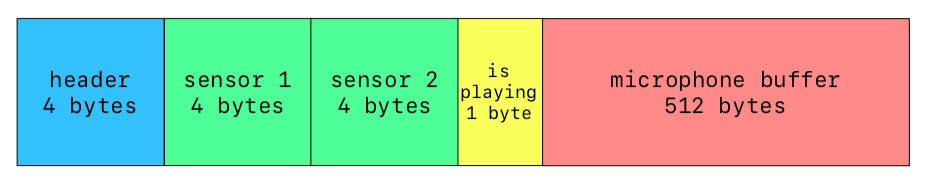
\includegraphics[width=15cm]{images/packet.png}
\caption{структура пакета данных}
\end{figure}

В конце функции \verb|loop()| пакет данных отправляется на компьютер по USB:
\begin{lstlisting}
SerialUSB.write(packet, packet_length);
\end{lstlisting}

\subsubsection{Установка биболиотек для Arduino}

Также, данная программа для Arduino требует установки следующих библиотек. 

Во первых, нужно установить \texttt{arduino-cli} - с помощью этого инструмента производится загрузка программ на Arduino. Установочные файлы под разные операционные системы можно найти по ссылке https://github.com/arduino/arduino-cli во вкладке releases.

Установка драйверов для платы (arduino-cli/README.md)

С помощью \texttt{arduino-cli} нужно установить библиотеки:

\begin{lstlisting}
arduino-cli lib install "DueTimer"
arduino-cli lib install "Adafruit BME280 Library"
\end{lstlisting}


Загрузка программы на ардуино производится с помощью скрипта \texttt{arduino.py}:
\begin{lstlisting}
python3 arduino.py _arduino
\end{lstlisting}


\begin{figure}[H]
\centering
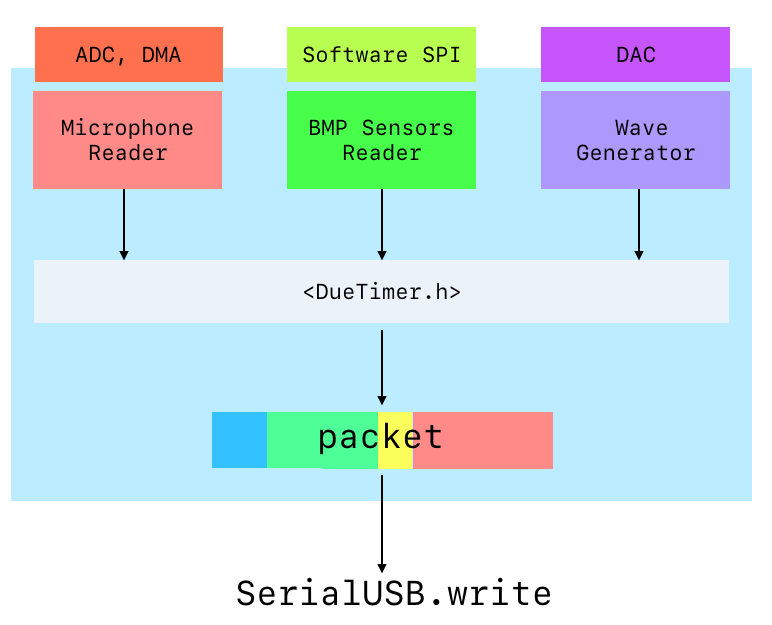
\includegraphics[width=\textwidth]{images/arduino-schema.png}
\caption{Диаграмма классов ПО для Arduino Due}
\end{figure}

\newpage

\end{document}
